\documentclass{article}
\usepackage{tikz}
\usetikzlibrary{automata,positioning}

\begin{document}

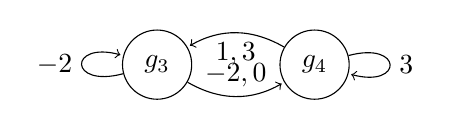
\begin{tikzpicture}[shorten >=1pt,node distance=2cm,on grid,auto]
    \node[state] (g3) {$g_3$};
    \node[state] (g4) [right=of g3] {$g_4$};

    \path[->]
        (g3) edge [loop left] node {$-2$} ()
             edge [bend right] node {$-2,0$} (g4)
        (g4) edge [loop right] node {$3$} ()
             edge [bend right] node {$1,3$} (g3);
\end{tikzpicture}

\end{document}